% Individual-Based Modeling (IBM)
%
% Advanced Project I - Jacobs University Bremen
% Supervisor: Dr. Stefan Kettemann
%
% Created on May 29, 2019
%
% Authors:
%   Ralph Florent <r.florent@jacobs-university.de>
%   Davi Tavares <davi.tavares@leibniz-zmt.de>
%   Agostino Merico <a.merico@jacobs-university.de>
%
% 1) Introduction
% 2) Theoretical background
% 3) Instrumentation (software and tools)
% 4) Methods (Procedure)
% 5) Results, Discussions
% 6) Conclusion
% 7) References

% ==============================================================================
% START: Methods, Results, Discussions, Conclusion
% ==============================================================================

\section{Theoretical Background}

\section{Instrumentation}

The VE, as specified literally, is developed in a complete \emph{virtualized} workspace. This virtualized workspace is made up of tools and software used to carry out this project to its current release. In this section, a brief overview of those tools and software is provided to help to reproduce or replicate the exact setup of the development environment put in place at the time of implementing the project.

\subsection{Tools and Software}
There are several currently-available programming tools that may achieve the same VE goal. The reason to believe so is that it turns out that today's open source community has grown larger and, subsequently, has been more actively involved in software improvements and new releases. As a result, accessing those online tools is no longer an issue, at least in terms of low-money budget, since they are publicly available (under free or moderately limited license).

Given the availability of several options, enlisted below are the most regular choices of  tools and software for a developer with mere knowledge in programming:
\begin{itemize}
    \item GNU/Linux Ubuntu 16.04 (operating system)
    \item Visual Studio Code (text editor for the documentation)
    \item Git\footnote{Also available as a bash emulation for other platforms for free (e.g. Git Bash for Windows).} (version control)
    \item GitHub (web-based hosting service for versioning system)
    \item Python (programming language for the scripting)
    \item Jupyter Notebook (workspace for the VE simulation)
\end{itemize}

\noindent
Obviously, it is not a concern to access and use a set of randomly compatible versions of the above-mentioned tools and software. However, in case a developer wants the exact versions, Table \ref{table:tools-and-software} lists more detailed information on both the versions and sources for future downloads.

\begin{table}[!ht]
    \begin{center}
        \begin{tabular}{ |l|l|l|l| }
            \hline
            \multicolumn{4}{ |c| }{ \textbf{Tools \& Software}} \\
            \hline % Table headers
             & \textbf{Version} & \textbf{Source} & \textbf{Cost}  \\ [0.5ex]
            \hline % Table body (row-wise contents)
            \textbf{\textit{Visual Studio Code}} & 1.34.0 & See link in [1] & Free  \\
            \hline
            \textbf{\textit{Git}} & 2.7.4 & Built-in Linux program & Free  \\
            \hline
            \textbf{\textit{GitHub}} & N/A & See link in [3] & 5 free users  \\
            \hline
            \textbf{\textit{Python}} & 3.5 & See link in [4] & Free  \\
            \hline
            \textbf{\textit{Jupyter Notebook}} & 5.7.4 & See link in [5] & Free  \\
            \hline
        \end{tabular}
        \caption{Detailed information on the tools and software used for the VE}
        \label{table:tools-and-software}
    \end{center}
\end{table}

\subsection{General Comments}
The tools and software discussed in the previous subsection are chosen by a matter of personal preference. No further comparison or parallelism procedure has been carried out to assess the most convenient option. That is to say, it might exist a better work environment where the VE simulation is simpler and/or easier, or the VE surprisingly performs better\footnote{In the outlook section, "simpler" and "easier" simulation is explained with the perspective of an ideal use case scenario. Similarly, a better performance of the VE refers to reduction in processing time, resource consumption in an easy-to-follow simulation platform.}. But, given that this first release is most importantly seen as a prototype, more tools and software can be tested out in a near future so that we end up with a so-called optimal workspace for the VE.

\section{Methodology}
This section will explore the methods used to implement the core functionality of this project. This exploration includes the mention of the workflow scheme, the third-party libraries usage and options, the algorithm and content structure, and finally the programmatically-implemented coding procedure.

\subsection{Workflow Scheme}
This project's workflow scheme consists of 3 main steps:
\begin{enumerate}
    \item \textit{Initialize}: stands for initial conditions
    \item \textit{Observe}: handles the graphical parts
    \item \textit{Update}: computes random movements based on the probability distribution of the corresponding factors.
\end{enumerate}
where each step contains itself a series of internal subprocesses aiming a specific goal.

\begin{figure}[h!]
    \centering
    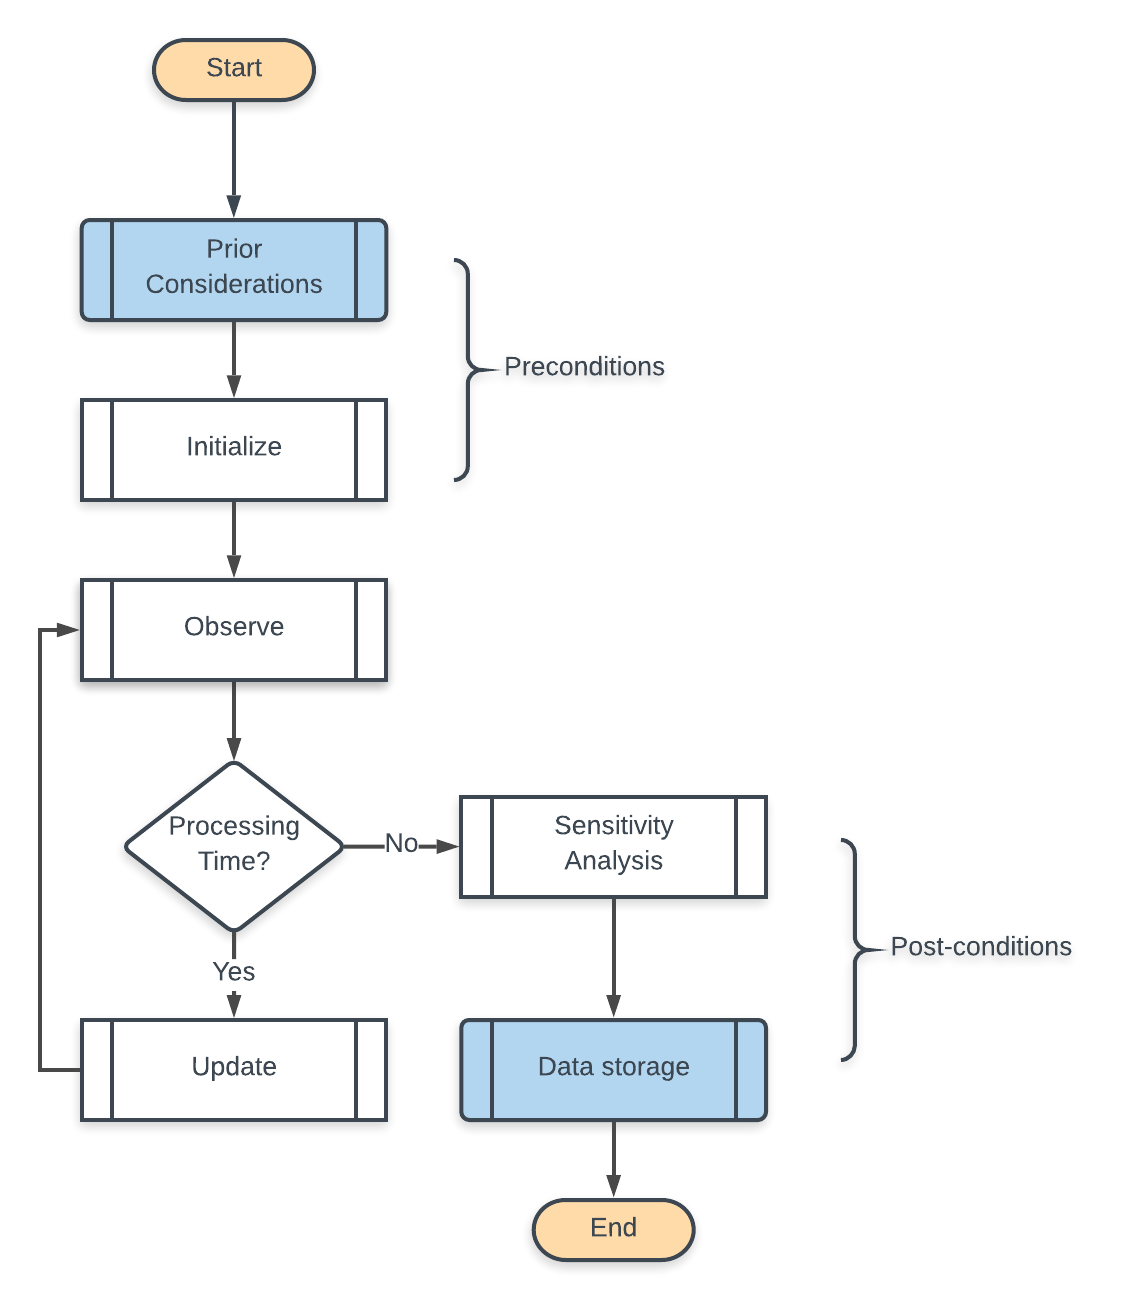
\includegraphics[scale=0.33]{workflow-scheme.png}
    \caption{Workflow diagram \\ (credits: made with \emph{Lucidchart})}
    \label{fig:workflow-scheme}
\end{figure}

\noindent
\textbf{Important}: Observe in Figure \ref{fig:workflow-scheme} the remaining steps categorized as \emph{Preconditions} and \emph{Postconditions}. They represent respectively the \emph{Before} and \emph{After} the 3 main steps \emph{Initialize, Observe, and Update} are executed. Note also that the \emph{Initialize} process is considered as part of the Preconditions semantics. That is because it only prepares the basic conditions for the components of the system, which are the habitats and the birds.

Analyzing the workflow diagram in Figure \ref{fig:workflow-scheme}, we denote the following fields:
\begin{itemize}
    \item \textbf{\textit{Start}}: indicates the starting point of the VE simulation.
    \item \textbf{\textit{Prior Considerations}}: are the basic setup necessary to fulfill the initialization phase requirements\footnote{These considerations, mostly based on the concerned entities (waterbirds, coastal lagoons), the environmental variables, and any additional properties contributing to the setup phase of the VE simulation, are also discussed in this document in the theoretical section.}. This setup spans the following elements: the geometry of the habitats and the human settlements; the functions defining the probability distribution of the random movements (driven by the water salinity, water depth, and food availability factors); the duration of the overall simulation process; and a reasonable threshold to handle the feasability of the random movements for a given seabird under certain conditions.
    \item \textbf{\textit{Initialize}}: creates the initial conditions of the system based on prior considerations mentioned above. That is, the patches (habitats) and agents (seabirds) creation.
    \item \textbf{\textit{Observe}}: generates a 2-dimensional plot whose scale goes from zero to one(\emph{$0-1$}) in both axes (x, y). The rendered plot helps to visualize both the patches' and agents' positions.
    \item \textbf{\textit{Processing Time?}}: focuses on updating the agents' positions' as long as the conditional parameter for the processing time holds. That is, the iteration is exclusively based on a specific number of times without accounting for other parameters that might influence the habitats and the birds. Note that, in this current version, the iteration is set statically during the prior considerations process.
    \item \textbf{\textit{Update}}: randomly assigns an agent to new positions within the existing habitats, considering a given threshold and the other aspects of the probability distribution.
    \item \textbf{\textit{Sensitivity Analysis}}: collects the probability values to form a set of probability distributions, which later can be analyzed and compared to each other with the expectation to draw conclusions on the final output.
    \item \textbf{\textit{Data Storage}}: given the generated plots, collects  them as PNG images and then generates a GIF out of the entire dumped images. This is relevant to provide the end-user useful insights on the collected data.
    \item \textbf{\textit{End}}: indicates the ending point of the VE simulation.
\end{itemize}

Recalling that this Virtual Environment constitutes essentially a digital representation of an Agent-Based Modeling system, each component of such a system relies on the interaction and interconnection with other involved components in an organized flow. Therefore, the diagram in Figure \ref{fig:workflow-scheme} shows a workflow scheme that intends to provide with a visual aid for a better understanding of the system's behaviour.

\subsection{Third-Party Libraries}

\subsubsection{Usage}
\subsubsection{Options}

\subsection{Algorithm \& Data Structure}

\subsection{Implementation}

\section{Results \& Discussions}

\section{Conclusion}

% ==============================================================================
% END: Methods, Results, Discussions, Conclusion
% ==============================================================================